\section{Block Diagrams} % overview + VRAM

\begin{figure}[ht!]
    \centering
    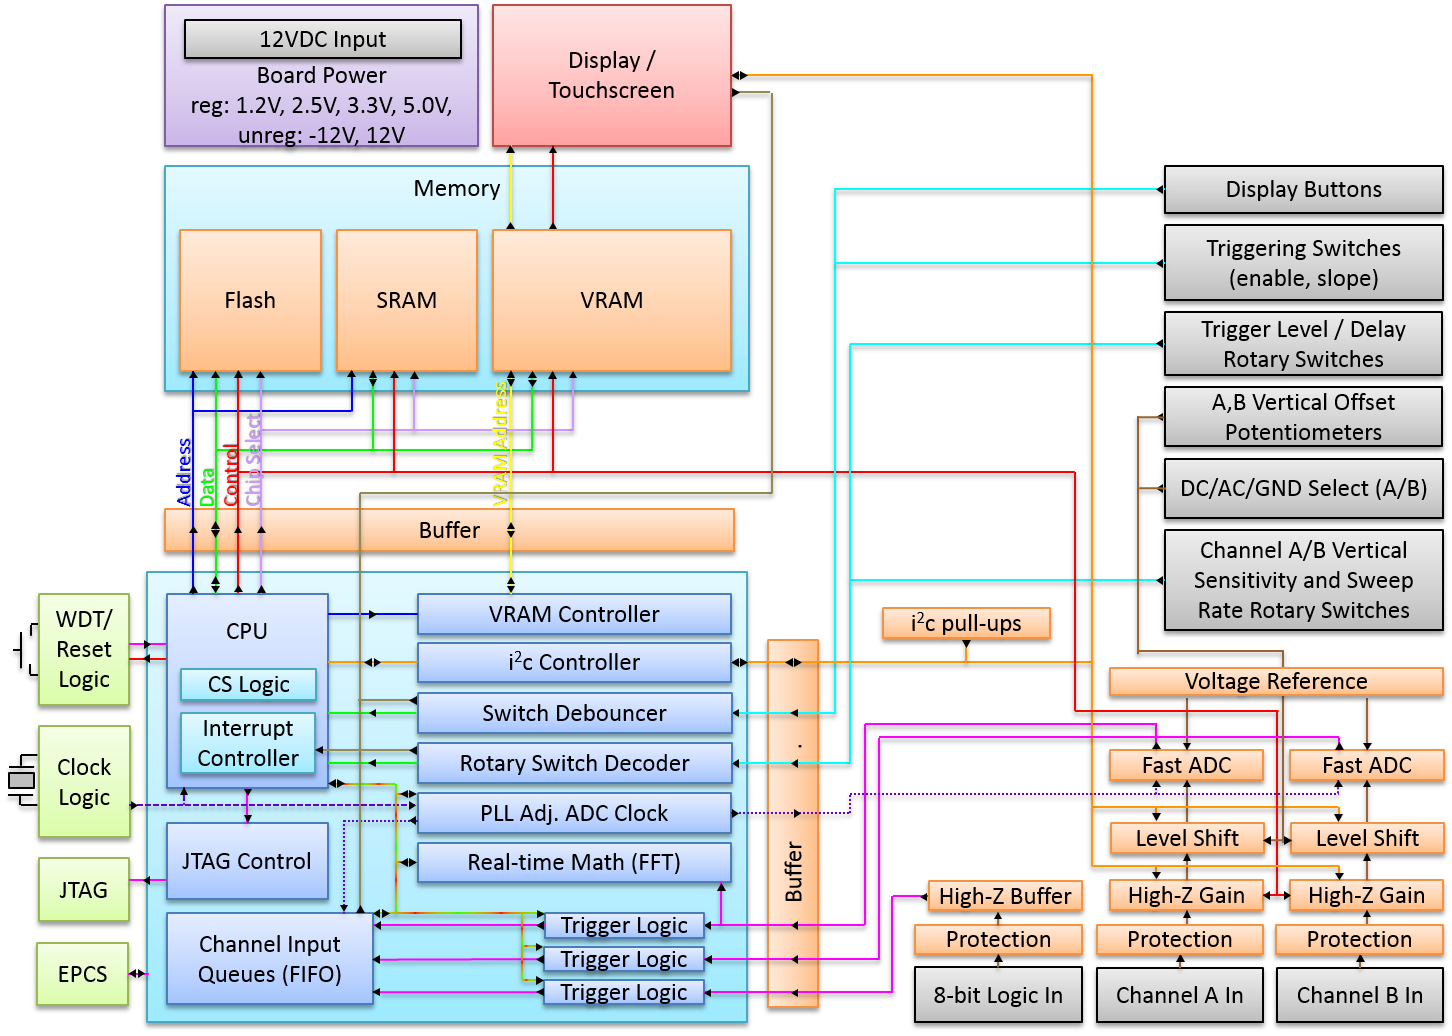
\includegraphics[width=6in]{block_diagrams/full.png}
		\caption{Full block diagram}
\end{figure}

The hardware consists of four main modules: the FPGA (and supporting hardware), the analog input, the memory devices and display, and the switches. On the block diagram above, the FPGA components are in the bottom left with the FPGA itself represented by the large light blue rectangle, the analog is in the bottom right, the memory is in the top left, and the switches are in the top right.

The FPGA itself consists of several separable components, although these will be covered more in the Firmware section (Chapter \ref{firmware}). As a broad overview, the FPGA features a soft-core CPU, a controller for the VRAM and display, logic for handling switch and rotary encoder input, and the entire ADC input and triggering section. As seen in the block diagram, all of these major components have inputs and outputs to the other major hardware components of the board; they are also all buffered to protect the FPGA.

The analog section consists of two analog channels (A and B) and an 8-bit logic analyzer. While the logic analyzer feeds directly to the FPGA buffer inputs, the two analog channels are fed through an analog front-end before being converted by the ADC. The analog front-end supports a large range of input voltages due to the input protection and voltage scaling op amp circuits. The front-end also contains a few user-controls: the voltage can be shifted using the voltage shift potentiometers; the input mode can be selected between DC, AC, and GND. While the gain is also variable as a function of the vertical sensitivity rotary encoders, the control is indirect (through the FPGA/CPU) as opposed to being a direct part of the analog circuitry.

The memory consists of three separate components: the flash, the SRAM, and the VRAM (plus display). These are connected to the FPGA's soft core CPU as you might expect: address and data buses, as well as chip select and read/write lines. One thing to note is that the VRAM has a separate address bus (9 bits), whereas the flash and SRAM share a 16-bit address bus. The flash memory serves as a non-volatile memory for storing the soft core CPU's operating system. The SRAM serves as external storage for the CPU. The VRAM is memory for the display, discussed in more detail below.

Finally, the user interface is controlled by a number of switches and rotary encoders / potentiometers. Some of these directly control the analog circuitry (potentiometers and mode select slide switches), while others indirectly control the board through FPGA logic (pushbutton switches and rotary encoders). Input from these switches is debounced or interpreted (for rotary encoders), then that simplified information is used to generate an interrupt for the CPU. All debouncing and rotary encoder decoding is done in the FPGA logic (not in the CPU's program).

\begin{figure}[ht!]
    \centering
    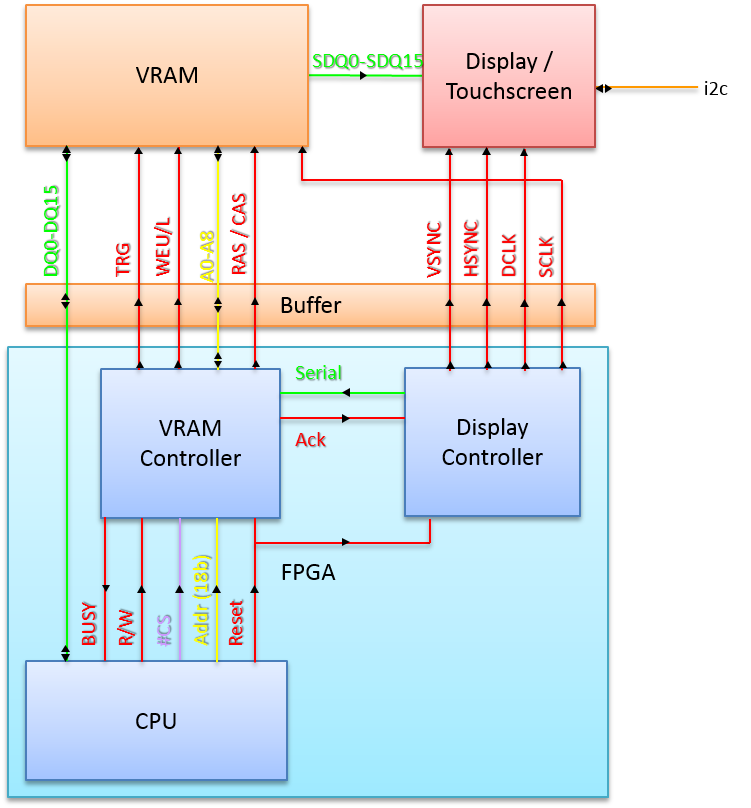
\includegraphics[width=3in]{block_diagrams/video.png}
		\caption{Display block diagram}
\end{figure}

This is a closer look at the VRAM / Display section of the hardware. The large containing blue block represents components internal to the FPGA, and the other blocks represent external components. As usual, there's a buffer to protect the FPGA from damage.

To read/write data to the VRAM (for eventual display by the display), first the CPU tries to write to the VRAM address of interest (18 bits), offset by the VRAM's location in the address map. This actually sends a signal to the VRAM controller (in FPGA logic) that splits the address into the row and column (9 bits each). The VRAM controller sends out the proper signals to the external VRAM chip, allowing the CPU to read or write data. Thus, the VRAM controller and VRAM together form, what looks like to the CPU, a single standard memory component.

With the VRAM loaded with display data, the display should be updated to show what's in VRAM. This operation is done completely separate from the CPU (all in FPGA logic) with the display controller. The display is a parallel input device which takes three clocks (VSYNC, HSYNC, DCLK), which will be discussed in more detail later. At each of the dot clocks, the parallel input takes a color for what to display at the current dot. Thus, the VRAM must output (SDQ0-15) to the display each pixel as requested - the VRAM is clocked by (SC).

The combination of CPU reads/writes to VRAM and VRAM serial transfers to display completes the operation of the display subcomponent of the hardware.

\section{FPGA}

\begin{figure}[ht!]
    \centering
    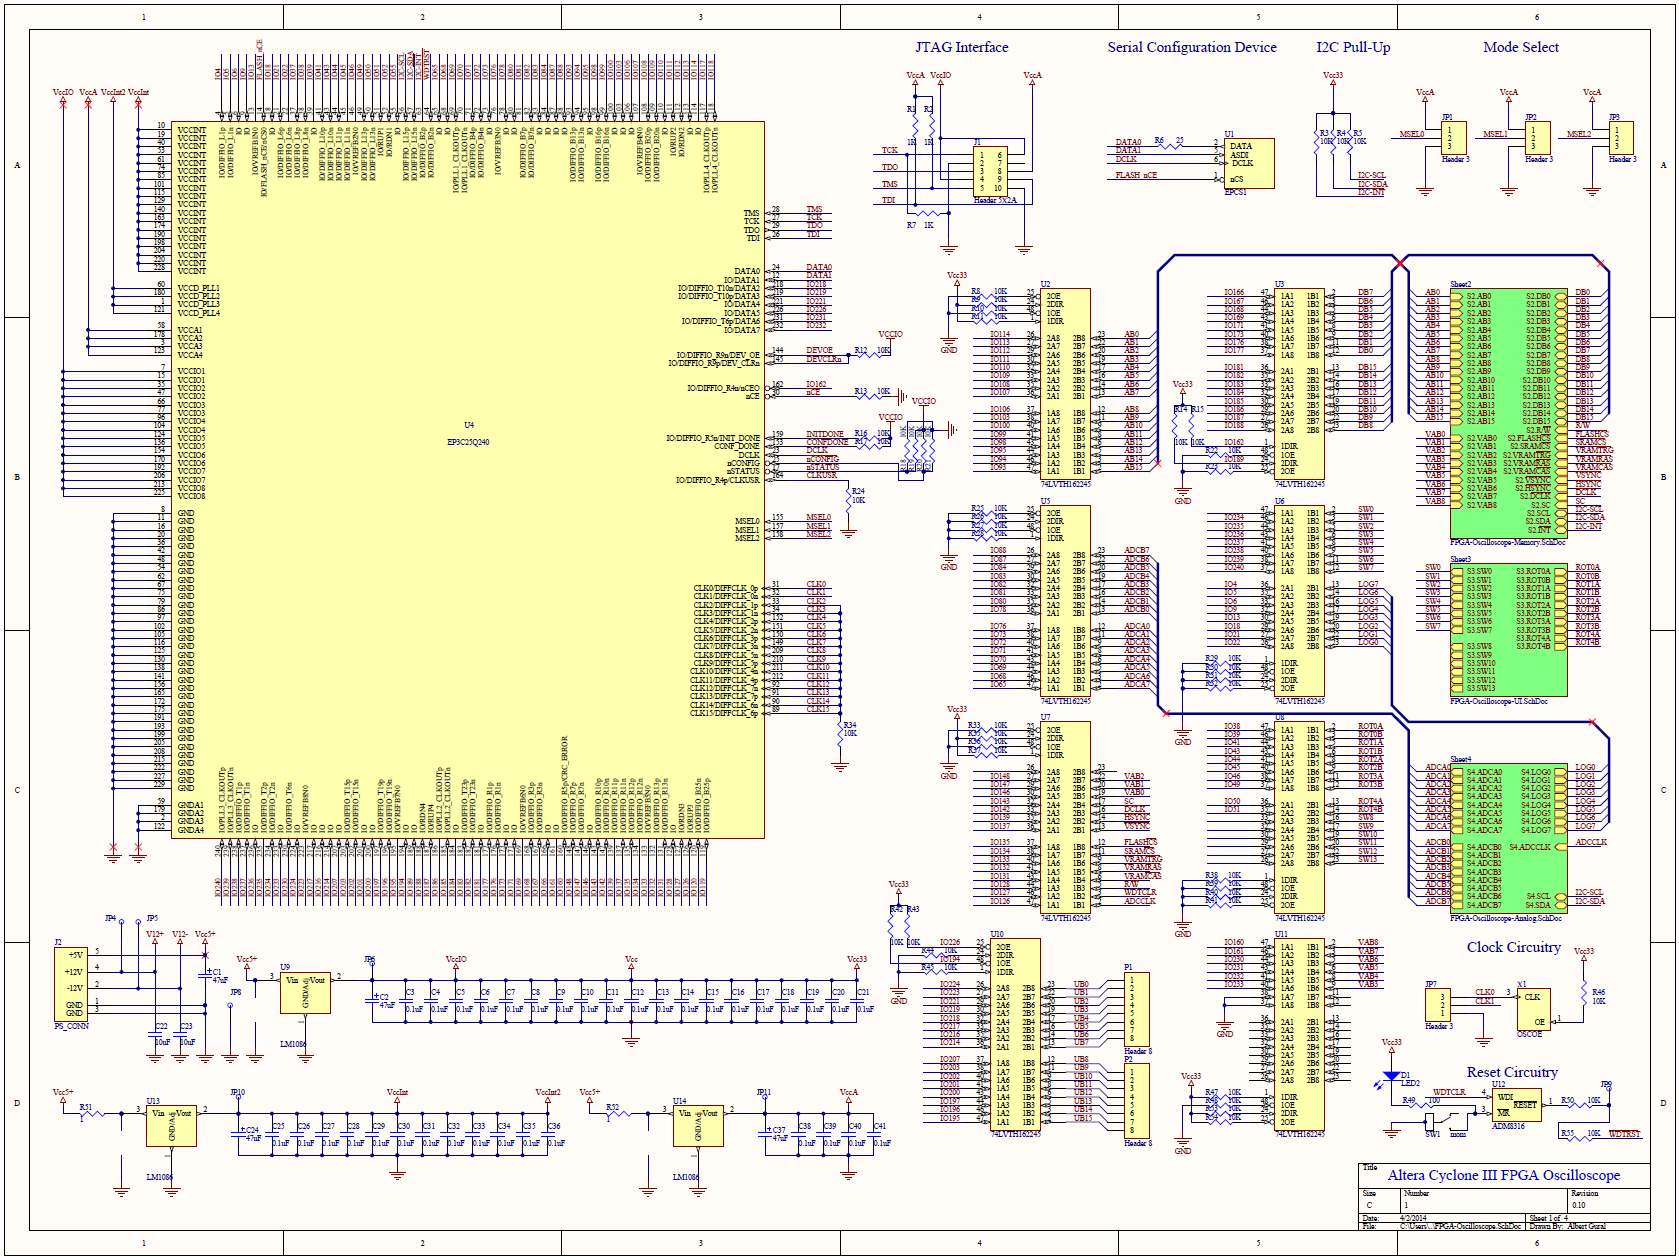
\includegraphics[width=6in]{circuit/main_fpga.png}
		\caption{FPGA and supporing components schematic diagram}
\end{figure}

The FPGA is a Quartus EP3C25Q240 Cyclone III FPGA (240-pin quad flat pack) [U4]. Besides various configuration pins, it contains a large number of general purpose I/O. These are connected through buffers [U2,3,5,6,7,8,10,11] to external circuit components.

Power for the entire board is provided by [J2] and contains dual $\pm 12V$ power, as well as a higher current $5V$ line. The FPGA operates on three voltages. The core is powered at $1.2V$ with [U13], the internal analog circuitry is powered at $2.5V$ with [U14], and the I/O banks are powered at $3.3V$ with [U9].

\section{FPGA Support}

There are a few other supporting components specifically for the FPGA. [J1] is a JTAG header that allows configuring the FPGA logic, as well as downloading code for the soft core CPU. [U1] is a serial configuration chip (EPCS16 with 16MB of space) which allows the FPGA to be re-configured after power is lost, without reprogramming the device through JTAG. [JP1-3] provide mode select capabilities. The board is typically kept in Fast Standard Mode with $3.3V$. [X1] provides a $36MHz$ clock signal. [U12] is a watchdog reset chip that can be used to automatically reset the FPGA (or just the CPU) in the case that the CPU stops operating or reaches an infinite loop.

\section{Analog Frontend}

\begin{figure}[ht!]
    \centering
    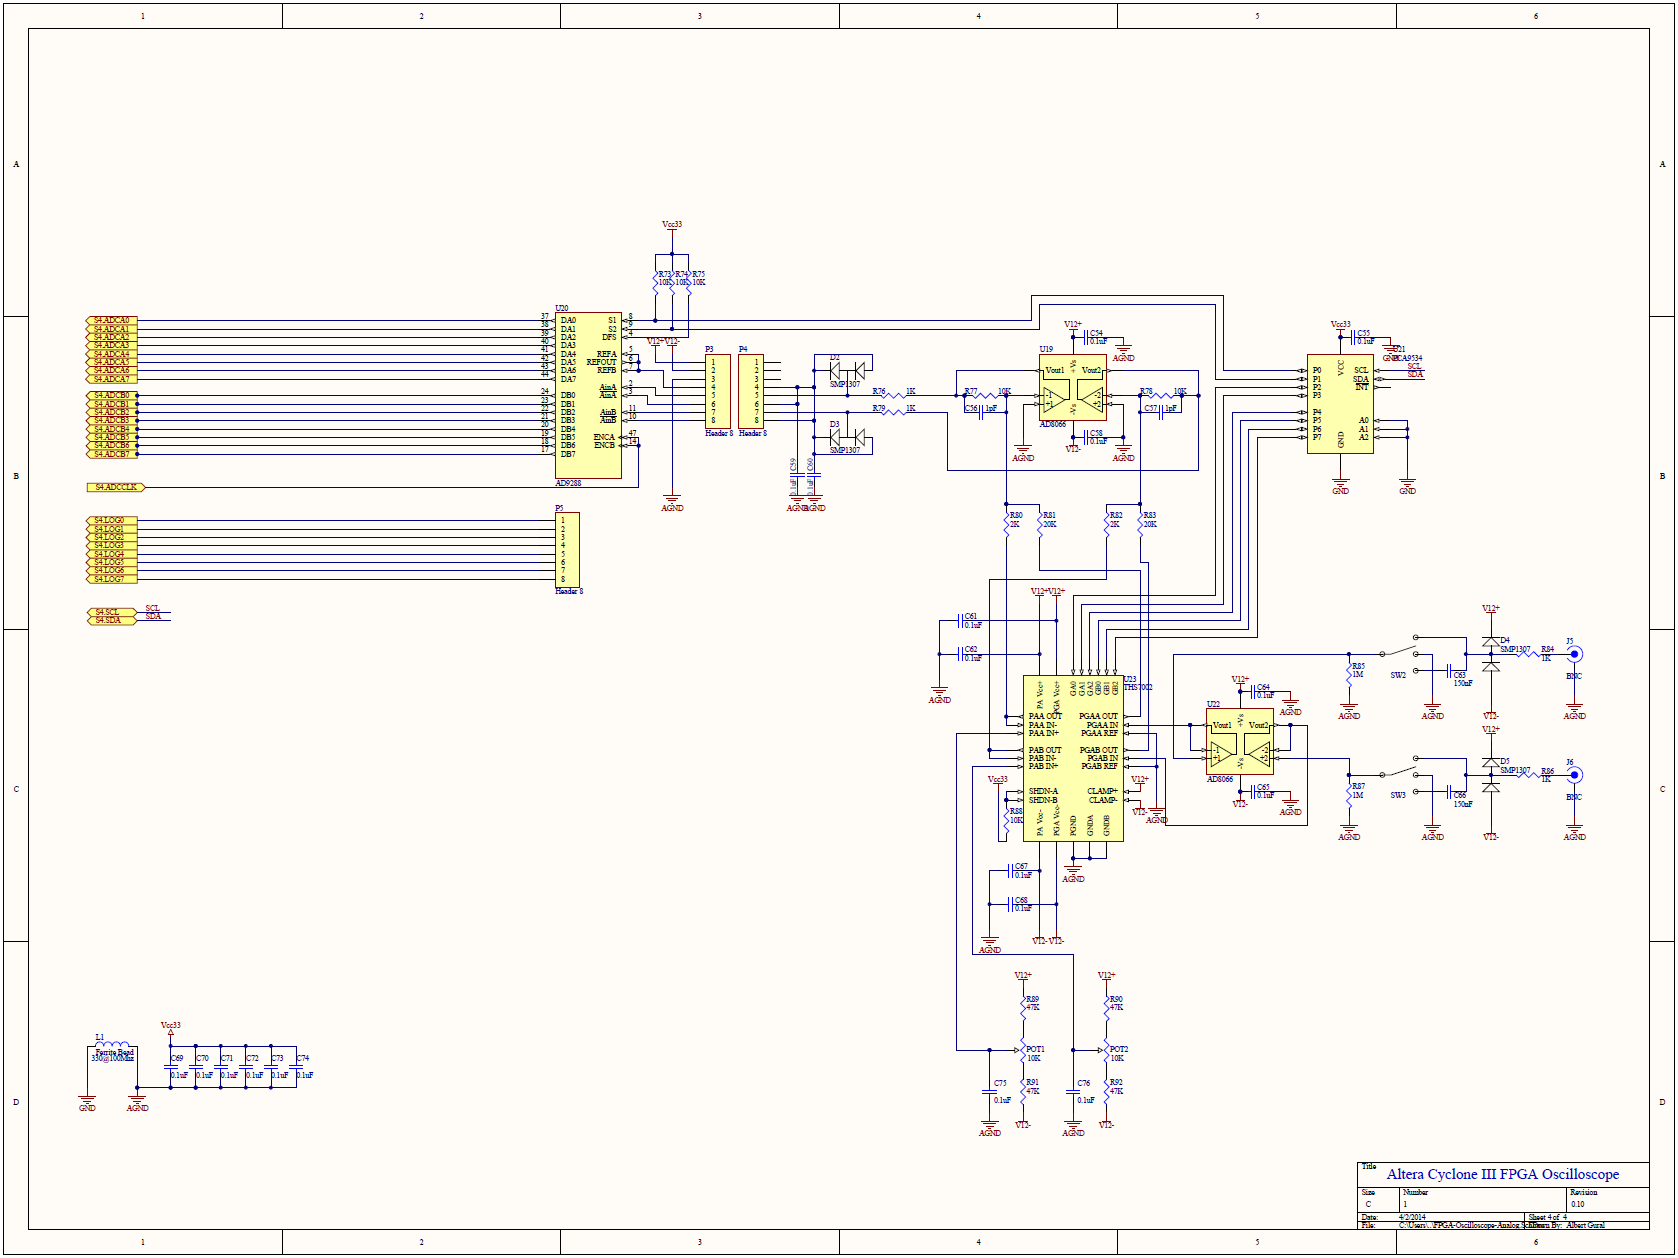
\includegraphics[width=6in]{circuit/analog.png}
		\caption{Analog section schematic diagram}
\end{figure}

The analog section contains two channels (A and B) for dual analog input capabilities. Starting from the BNC connector inputs, we can see the full path the signal takes before reaching the ADC to be collected digitally by the FPGA.

BNC connectors [J5-6] take analog input from a standard oscilloscope probe (or a 10x probe). Diode packages [D4-5] provide protection from excessive voltages. [SW2-3] allows for selection of the input mode (between DC/AC/GND). From there, the signals are buffered with [U22], then fed into a programmable gain amplifier (selectable -20dB to 20dB gain) [U23]. [U21] is an extended i2c controllable I/O port which allows for selecting the desired gain on the PGA.

From the PGA, the signal passes through another high-Z buffer [U19], which also provides level shifting (the shift level is provided by potentiometers [POT1-2], which are analog buffered by unused preamplifiers in the PGA [U23]). Finally, the output is again protected by safety diodes before reaching the ADC. Because the ADC has a voltage input swing of $\pm 0.512V$, the $0.7V_F$ diodes [D2-3] can be connected as shown to provide decent protection. They essentially limit the ADC input to within $0.7V$ of the reference voltage.

[U20] is the ADC, which provides 8 bits of data for each of the A and B channels. [P5] is a header for providing 8 bits of logic-analyzer input.

\section{Analog Frontend Transfer Properties}

Effort was put forth to make sure the analog front-end (at least at near-unity gain) had decent transfer function characteristics. Ideally, at least a $5MHz$ bandwidth and no ringing. There were issues, initially, with ringing, as seen in the left of the image below. However, fine-tuning [C56] and [C57] turns out to allow for the results seen in the middle and right.

\begin{figure}[ht!]
    \centering
    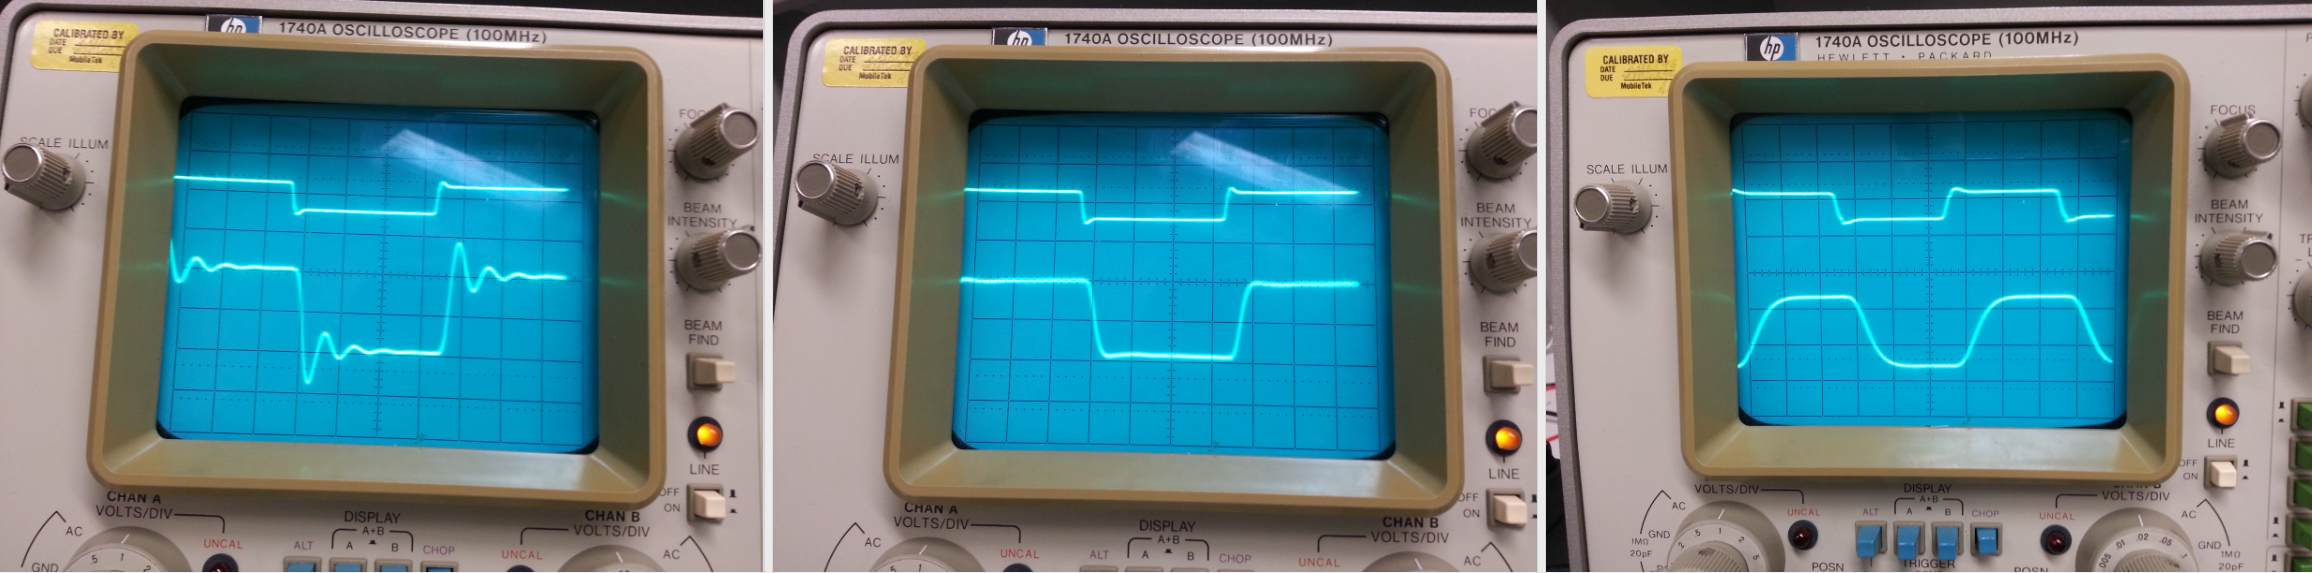
\includegraphics[width=6in]{specs/tuning.png}
		\caption{Analog frontend step response (input top; output bottom). The left is an underdamped response [C56] $= 0pF$, the middle is well-damped [C56] $= 2pF$, and the right is overdamped [C56] $= 5pF$.}
\end{figure}

With the $2pF$ values chosen, measurements of the gain and phase were made at a wide range of frequencies. From the step response, we can tell that the circuit has a nice transfer function, but this allows for a more quantitative characterization. Here are the results (DC input mode, -$6dB$ low/mid-band gain):

\begin{table}[ht!]
	\begin{center}
	\caption{Transfer gain and phase at various frequencies}
	\begin{tabular}{|c|c|c|}
		\hline
		Frequency & Gain & Phase \\ \hline
		$0.1Hz$ & $-5.7 dB$ & $0^o$ \\ \hline
		$0.2Hz$ & $-5.7 dB$ & $0^o$ \\ \hline
		$0.5Hz$ & $-5.7 dB$ & $0^o$ \\ \hline
		$1.0Hz$ & $-5.7 dB$ & $0^o$ \\ \hline
		$\vdots$ & $\vdots$ & $\vdots$ \\ \hline
		$5kHz$ & $-5.7 dB$ & $0^o$ \\ \hline
		$10kHz$ & $-5.7 dB$ & $0^o$ \\ \hline
		$20kHz$ & $-5.7 dB$ & $0^o$ \\ \hline
		$50kHz$ & $-5.4 dB$ & $0^o$ \\ \hline
		$100kHz$ & $-5.4 dB$ & $0^o$ \\ \hline
		$200kHz$ & $-5.4 dB$ & $-7^o$ \\ \hline
		$500kHz$ & $-5.4 dB$ & $-14^o$ \\ \hline
		$1MHz$ & $-5.2 dB$ & $-29^o$ \\ \hline
		$2MHz$ & $-5.4 dB$ & $-54^o$ \\ \hline
		$3MHz$ & $-6.0 dB$ & $-84^o$ \\ \hline
		$4MHz$ & $-6.7 dB$ & $-112^o$ \\ \hline
		$5MHz$ & $-8.0 dB$ & $-140^o$ \\ \hline
		$6MHz$ & $-9.4 dB$ & $-167^o$ \\ \hline
		$7MHz$ & $-11 dB$ & $-189^o$ \\ \hline
		$8MHz$ & $-13 dB$ & $-216^o$ \\ \hline
		$9MHz$ & $-15 dB$ & $-235^o$ \\ \hline
		$10MHz$ & $-18 dB$ & $-252^o$ \\ \hline
	\end{tabular}
	\end{center}
\end{table}

\newpage
This gives the following Bode plot:

\begin{figure}[ht!]
    \centering
    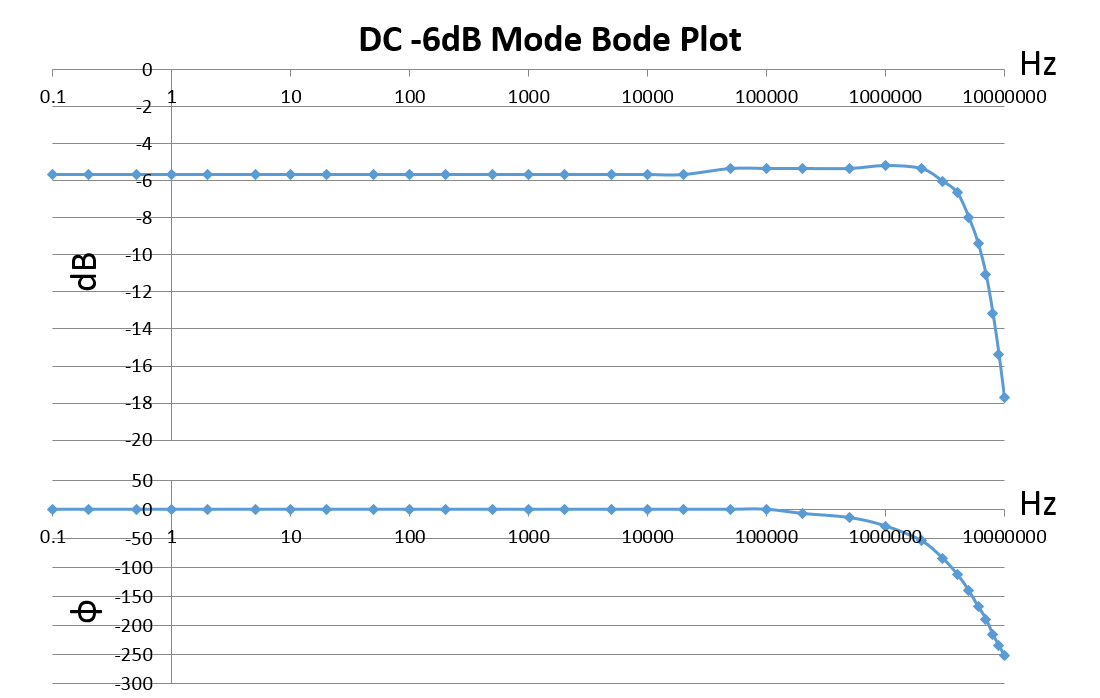
\includegraphics[width=4.5in]{specs/bode_raw.png}
		\caption{Analog input raw Bode plot}
\end{figure}

This gain and phase function is pretty good. Here's some additional analysis:

\begin{figure}[ht!]
    \centering
    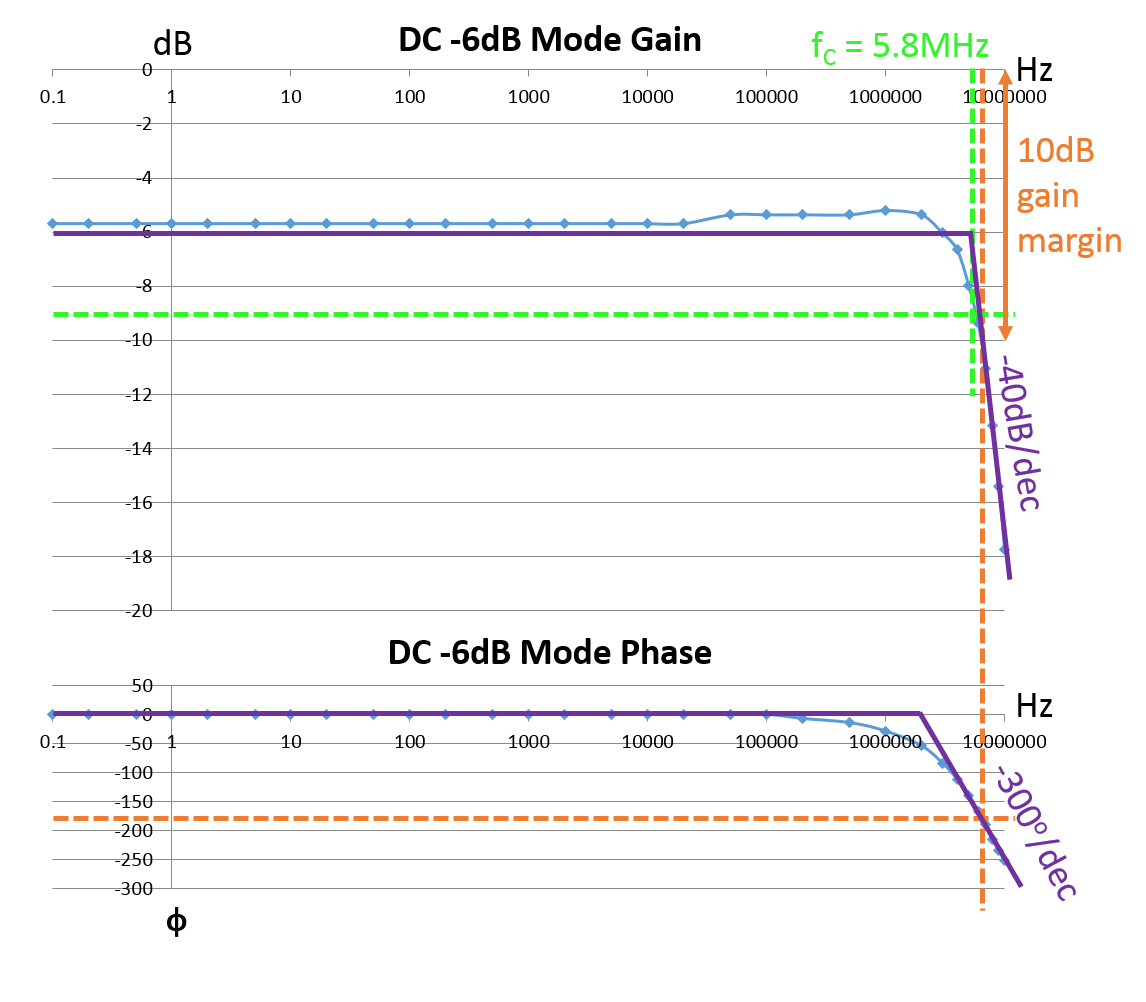
\includegraphics[width=4.5in]{specs/bode_total.png}
		\caption{Analog input Bode plot with annotations}
\end{figure}

As we can see, we achieve the desired $5MHz$ bandwidth with a corner frequency at $5.8MHz$.

\newpage
\section{ADC and Timing}

\begin{figure}[ht!]
    \centering
    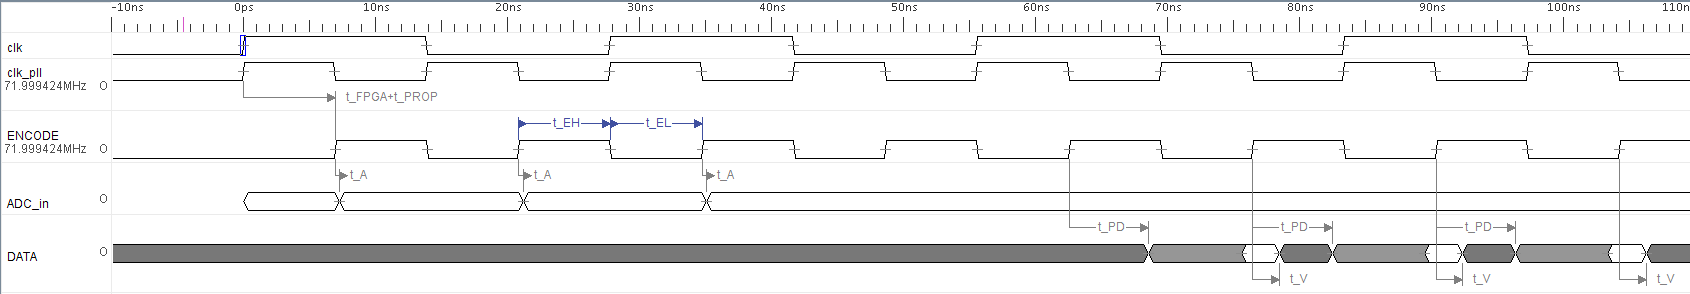
\includegraphics[width=6in]{Timing/FPGA-Oscilloscope-ANALOG.png}
		\caption{ADC timing}
\end{figure}

ADC timing is fairly straightforward. The FPGA provides a steady ADC clock (limited to a max of $80MHz$), which the ADC then uses to synchronously sample analog input and output the digital value. In the configuration shown, ADC channel A output is synchronized with the clock and channel B output is $180^o$ offset from that.

Because of the simplicity of timing and the fact that we don't care about small amounts of sample propagation delay, we can simply clock the FPGA sample collection synchronized with the ADC clock to get good data.

\section{Memory and Display}

\begin{figure}[ht!]
    \centering
    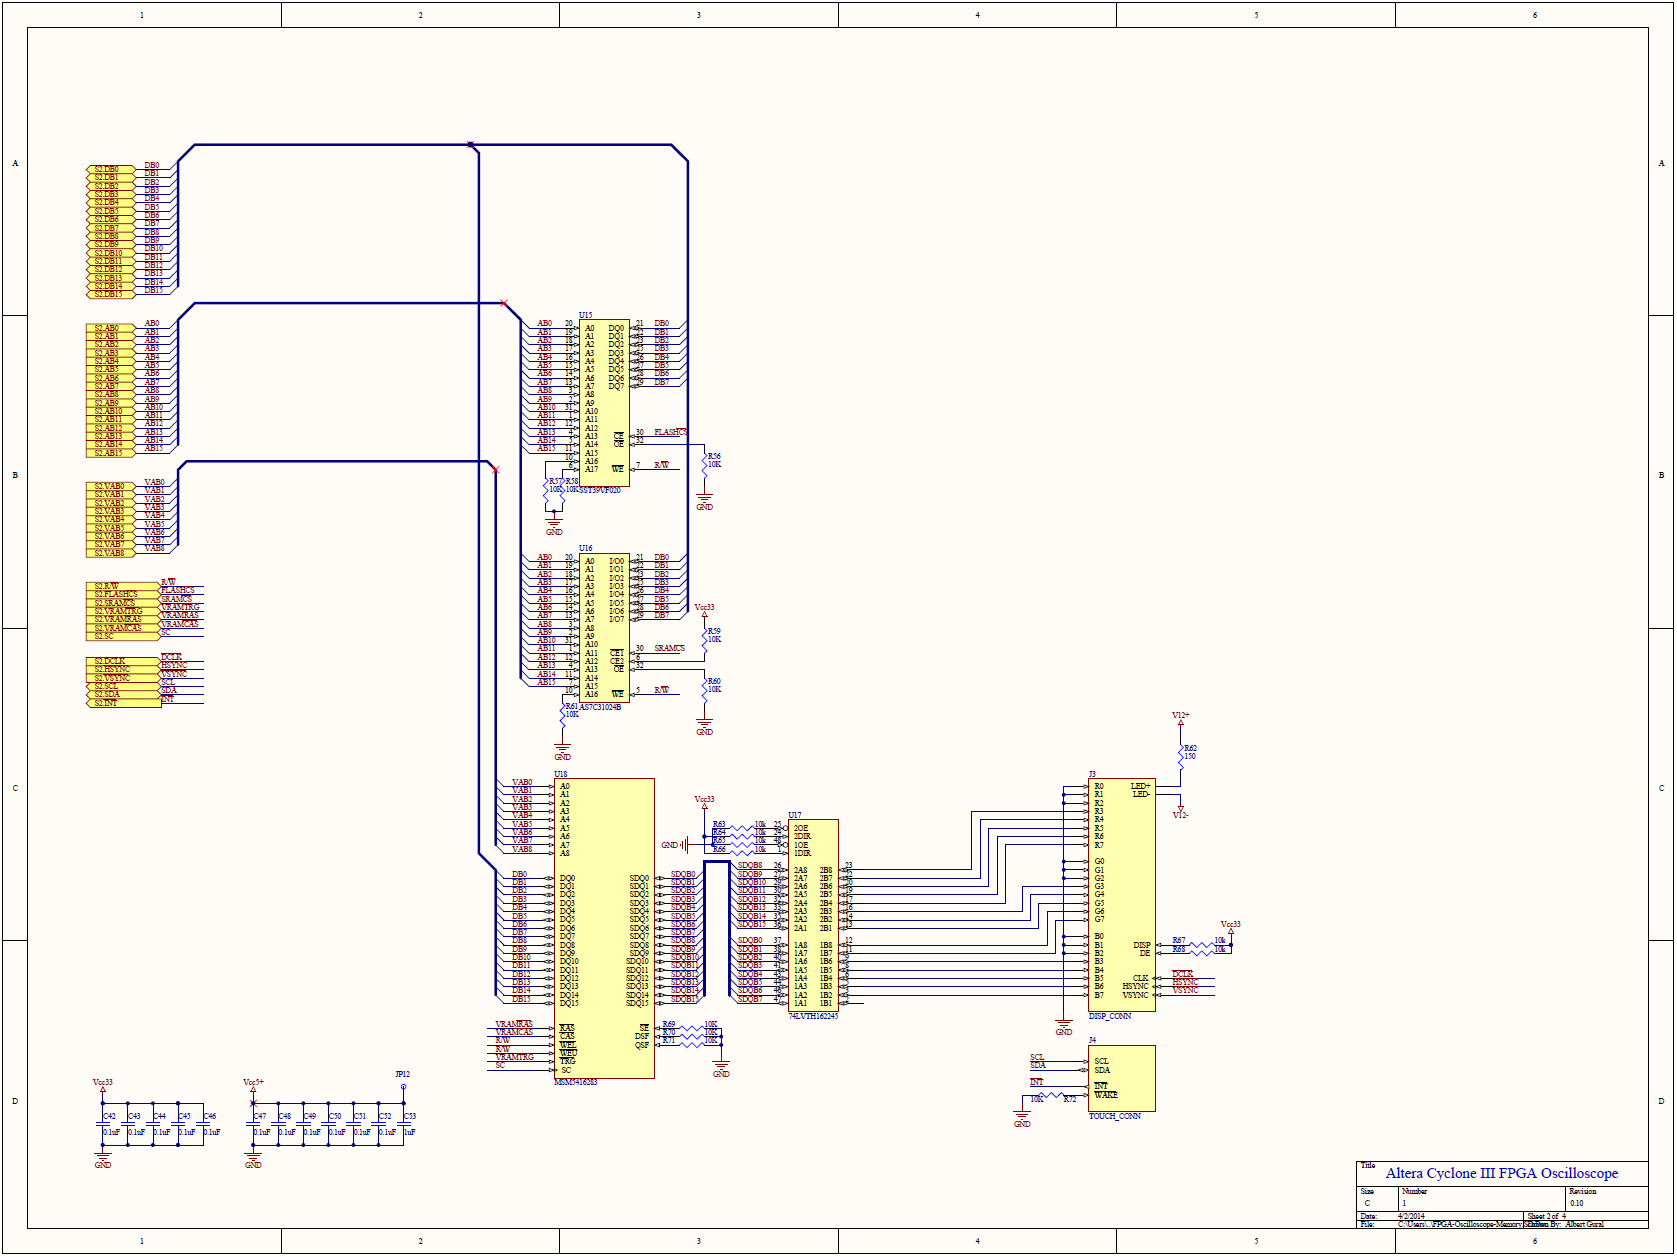
\includegraphics[width=6in]{circuit/memory.png}
		\caption{Memory schematic diagram}
\end{figure}

As discussed earlier, flash [U15] and SRAM [U16] are connected in fairly standard configurations. They share a data bus, address bus, and read/write line. Each has a separate chip select input. Both always have outputs enabled since we don't care about saving power.

While VRAM [U18] shares the same data bus and read/write line as flash and SRAM, it has its own 9-bit address line and two separate row/column chip selects. It also has a serial clock pin which outputs the next half-word of data to the SDQ line for the display (it should be clocked whenever we want to send a new pixel to the display). The VRAM operates at $5V$ while the display operates at $3.3V$, so [U17] provides necessary voltage level translation.

The display itself is a $480 \times 272$ 24-bit RGB display (connector [J3]) with a capacitive touch screen (and a controller that can be communicated with via i2c (connector [J4])). Because VRAM is only 16-bits, the system is only set up to control 5 bits of each color component (15-bit color control). The display is LED backlit (takes $19.2V$), so power is provided from the dual $\pm 12V$ line.

\section{SRAM and Timing}

\begin{figure}[ht!]
    \centering
    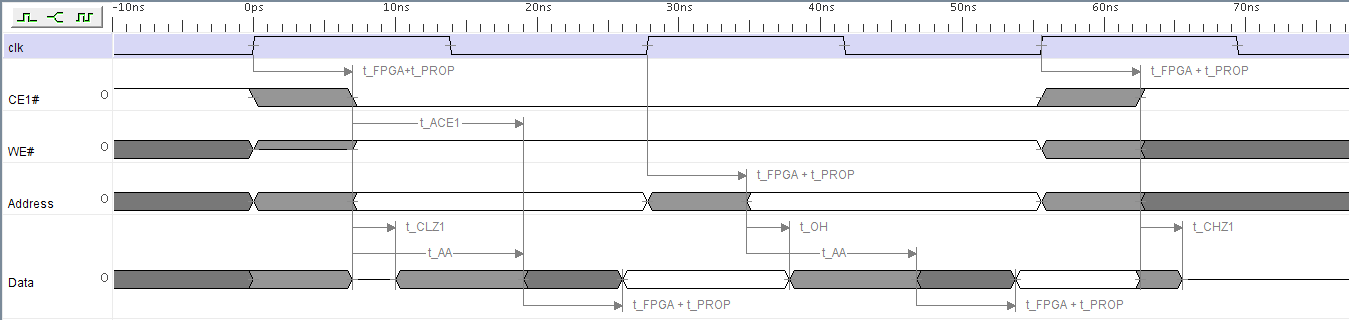
\includegraphics[width=6in]{Timing/FPGA-Oscilloscope-RAM-READ.png}
		\caption{SRAM read timing}
\end{figure}

\begin{figure}[ht!]
    \centering
    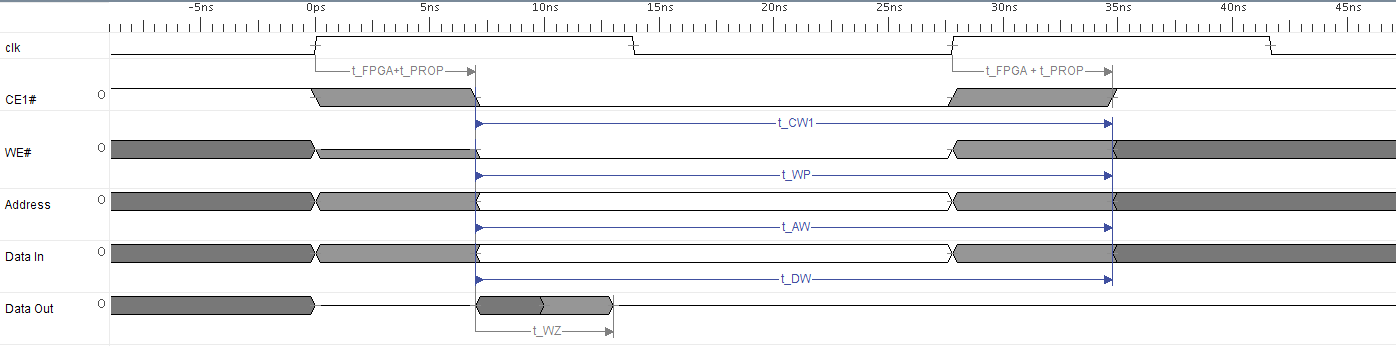
\includegraphics[width=6in]{Timing/FPGA-Oscilloscope-RAM-WRITE.png}
		\caption{SRAM write timing}
\end{figure}

SRAM timing is shown above. Since the FPGA is clocked with a $36MHz$ source ($27ns$ period), we can see that we can satisfy timing requirements if we have one clock cycle latencies for reading and writing, a one clock setup time, and a zero clock hold time.

\section{Flash and Timing}

\begin{figure}[ht!]
    \centering
    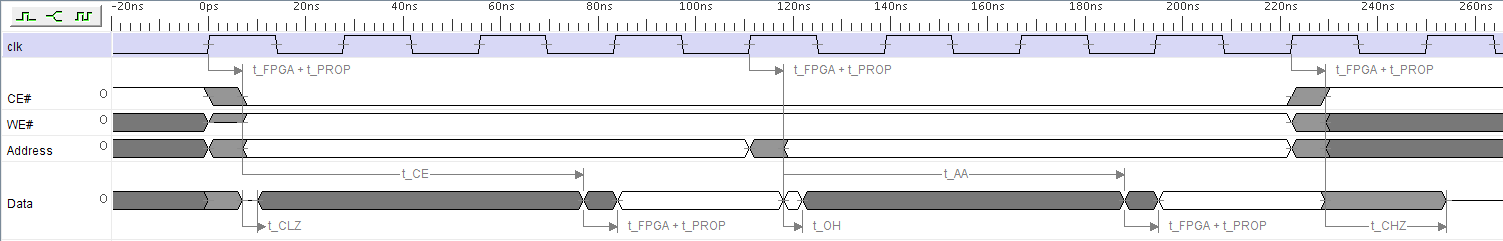
\includegraphics[width=6in]{Timing/FPGA-Oscilloscope-ROM-READ.png}
		\caption{Flash read timing}
\end{figure}

Flash timing is shown above. Since the FPGA is clocked with a $36MHz$ source ($27ns$ period), we can see that we can satisfy timing requirements if we have three clock cycle latencies for reading and no latencies for setup and hold times.

\section{VRAM and Timing}

Since VRAM is controlled by the VRAM controller, timing is important to understand what the VRAM controller must be capable of providing. The CPU, on the other hand, should interact with the VRAM controller using a busy signal. That is, after requesting a read or write, it will wait until the busy signal indicates the data can be read (if reading) or de-asserted (if writing).

The VRAM has four important operational modes. The first two, read and write, provide their obvious functionality. However, because VRAM is a DRAM, it requires period refreshes (refresh cycle). Finally, because it's a video RAM with one port for the CPU to read/write data and one port for the display to receive data, it also requires a serial row transfer cycle. During this cycle, data from a selected row is transferred to a special part of memory so that on serial clocks, the SDQ line fills with data from sequential memory cells in the selected row of memory.

\begin{figure}[ht!]
    \centering
    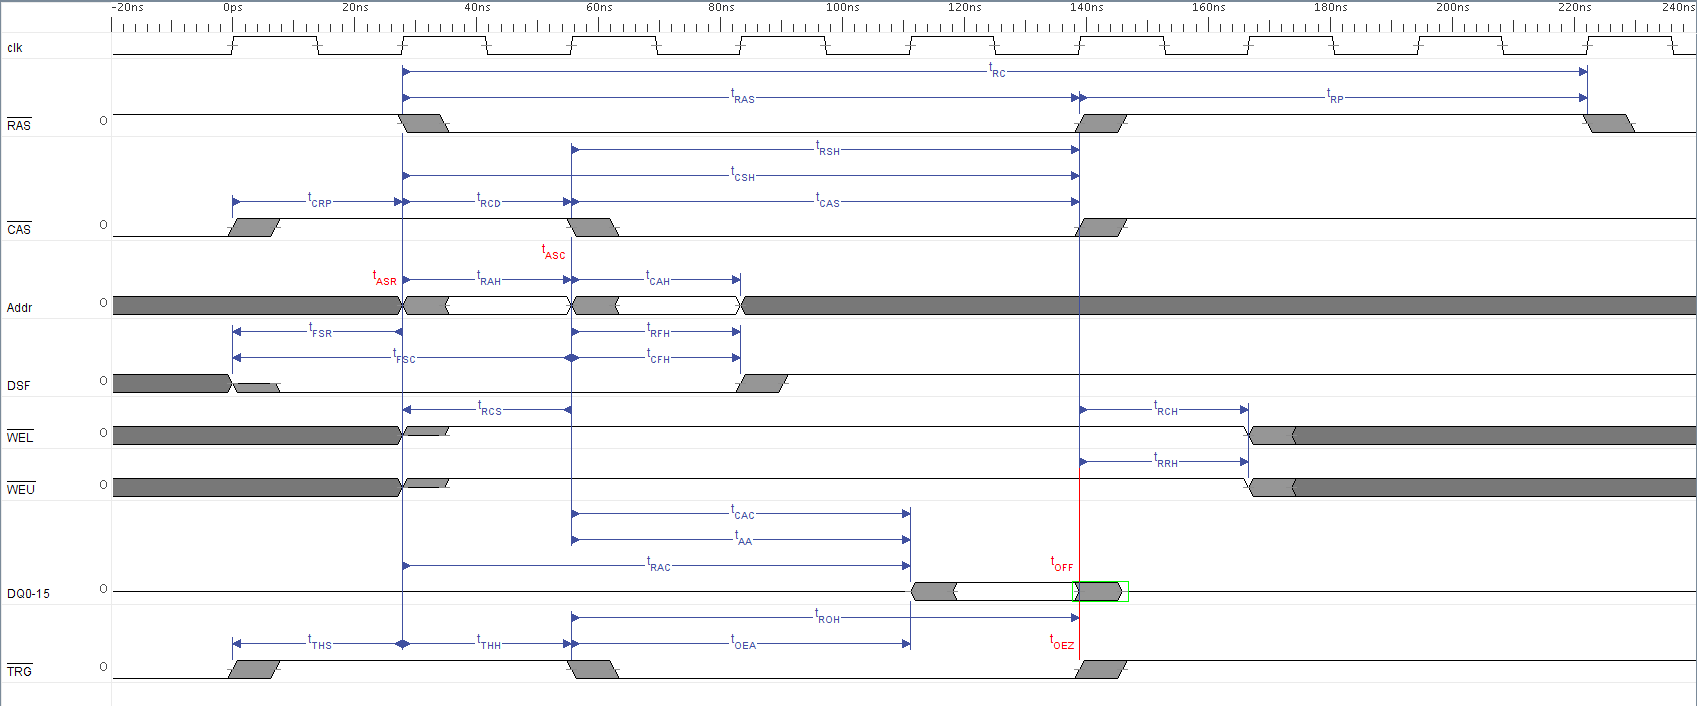
\includegraphics[width=6in]{Timing/FPGA-Oscilloscope-VRAM-READ.png}
		\caption{VRAM read timing}
\end{figure}

\begin{figure}[ht!]
    \centering
    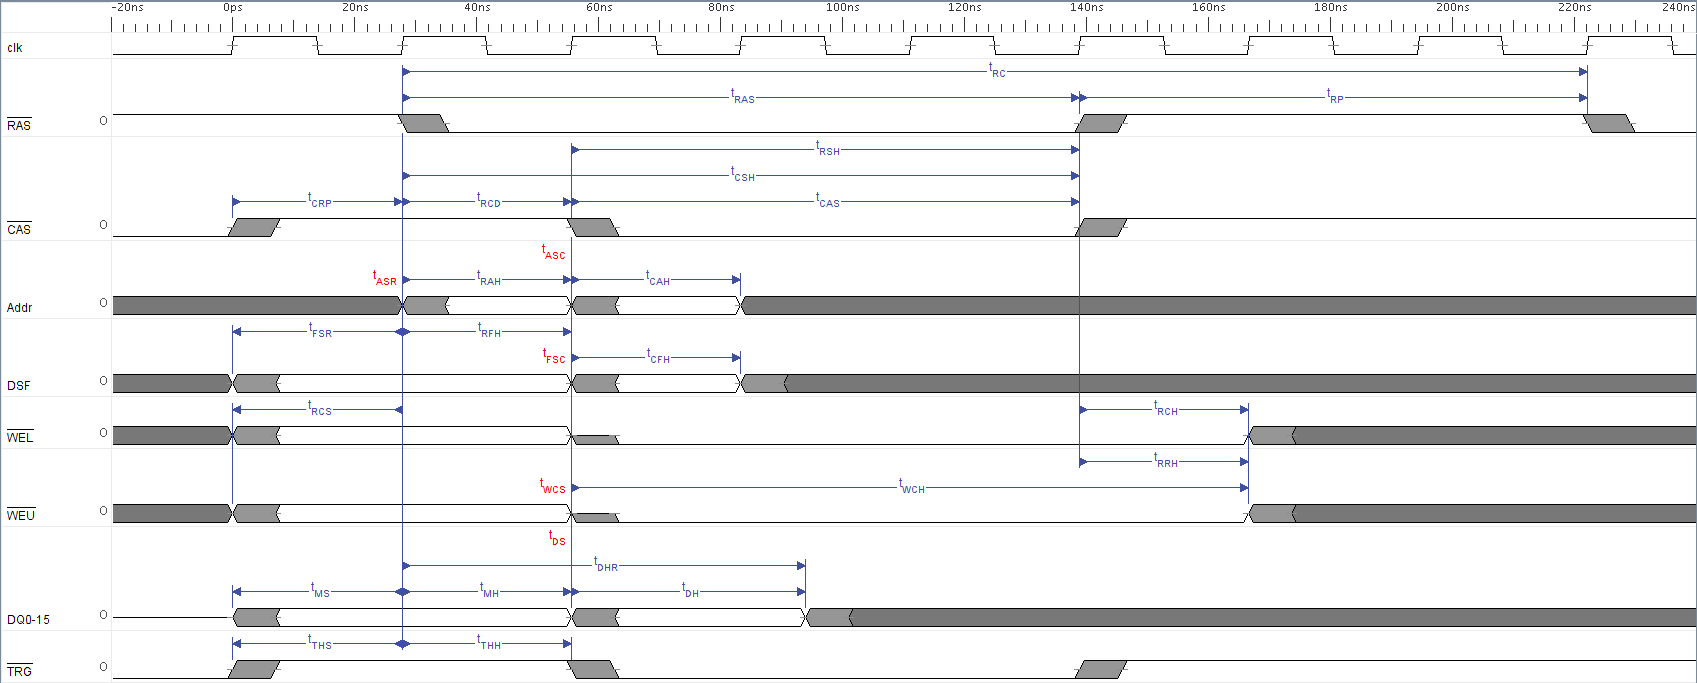
\includegraphics[width=6in]{Timing/FPGA-Oscilloscope-VRAM-WRITE-EARLY.png}
		\caption{VRAM early write timing}
\end{figure}

There are a fair number of signals at play, but the important ones for reading and writing are the address and data buses, the RAS/CAS signals, and obviously the read/write (WE) line.

\begin{figure}[ht!]
    \centering
    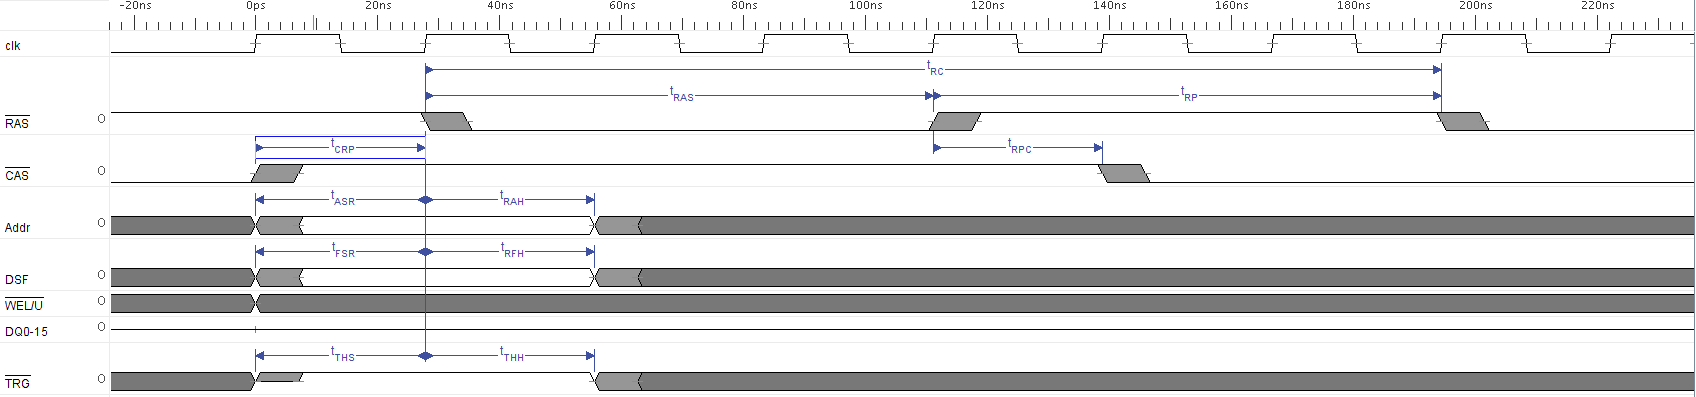
\includegraphics[width=6in]{Timing/FPGA-Oscilloscope-VRAM-REFRESH.png}
		\caption{VRAM refresh timing}
\end{figure}

A refresh cycle is typically very simple. The timing shown above is for a refresh cycle specific to a particular row. There's also a global refresh that refreshes the entire chip very quickly.

\begin{figure}[ht!]
    \centering
    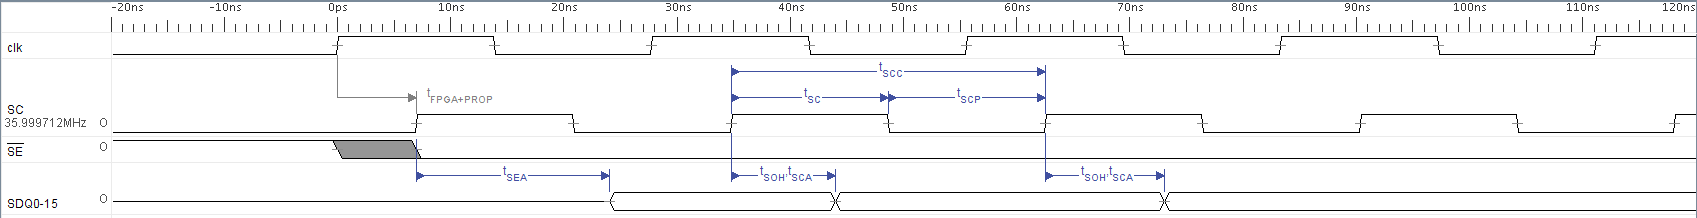
\includegraphics[width=6in]{Timing/FPGA-Oscilloscope-VRAM-SERIAL-READ.png}
		\caption{VRAM serial row transfer timing}
\end{figure}

The serial row transfer is also fairly simple. Simply provide the row of interest (the row that you want the display to update), and then provide the serial clocks to sequentially output data from that row.

With all of these timings, a state machine can be produced in FPGA logic that provides the necessary signals and delays to trigger the various VRAM modes. See the VRAM state machine VHDL code for more details on specific cycle delays for each of the modes.

\section{Display and Timing}

The display timing is shown below. The most basic timing is a steady dot clock (DCLK) that is the base pulse of all of the other pulses. During certain portions of the dot clock, each pulse sequences through a row of the display's pixels and any data on the parallel input is read as an RGB value for the display.

For each row to be displayed, there are front and back porches of a few dot clocks, during which nothing is changed on the display (this is shown on the bottom timing diagram). Each row is clocked by the HSYNC pulse. Many of these pulses allow for writing multiple rows of the display (as seen in the middle timing diagram).

Finally, when a screen's worth of rows are covered, the VSYNC pulses (as seen in the top timing diagram). Just as there were front and back porches for the dot clock with respect to a single HSYNC pulse, likewise there are front and back porches for the HSYNC with respect to a single VSYNC pulse. All of these front and back porches together forms an invisible frame around the true image during which the dot clock is active, but no new pixels are drawn to the screen.

\begin{figure}[ht!]
    \centering
    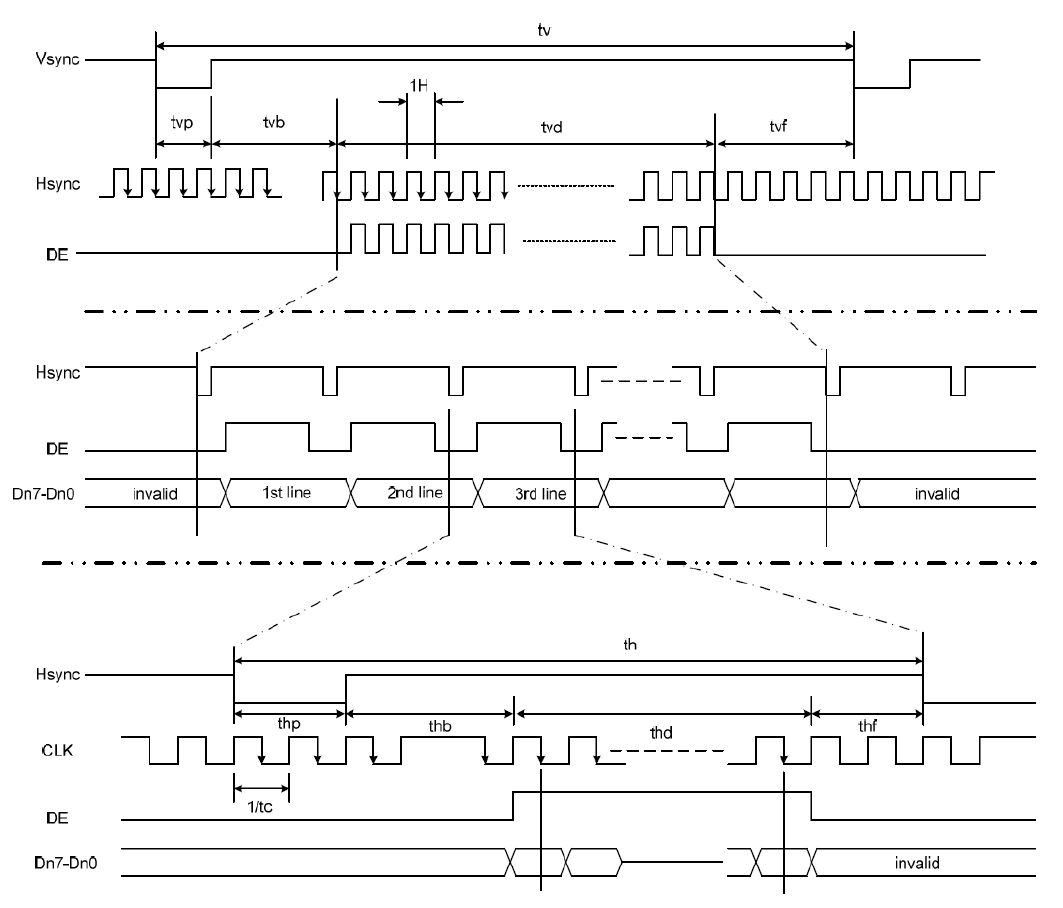
\includegraphics[width=6in]{Timing/disp_timing.png}
		\caption{Display timing}
\end{figure}

\begin{figure}[ht!]
    \centering
    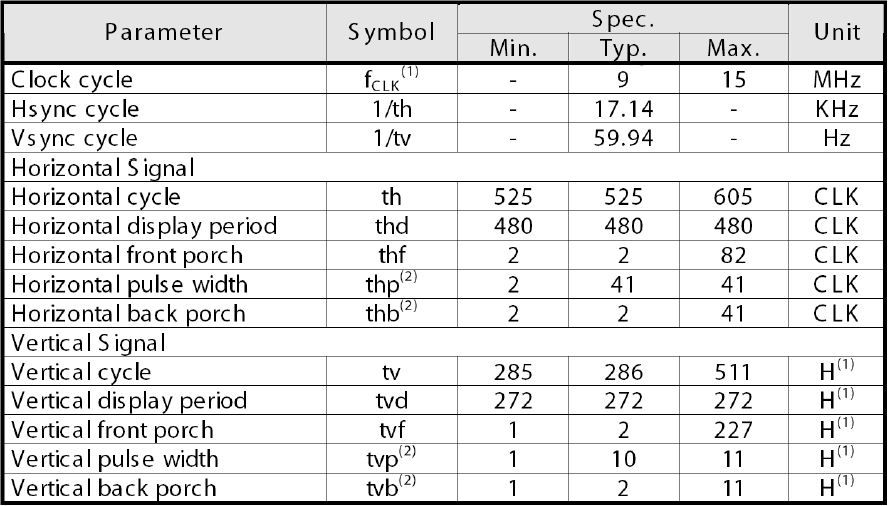
\includegraphics[width=3in]{Timing/disp_timing_chart.png}
		\caption{Display timing values}
\end{figure}

\section{User Input / Switches}

There are three different types of switches used on the board. Five momentary pushbutton switches are used as the screen menu select buttons. Two latching pushbutton switches are used for triggering controls (slope and trigger mode). Finally, five rotary encoders are used - two for the channel A/B vertical sensitivities, one for the time sensitivity, and two for trigger delay and level.

\begin{figure}[ht!]
    \centering
    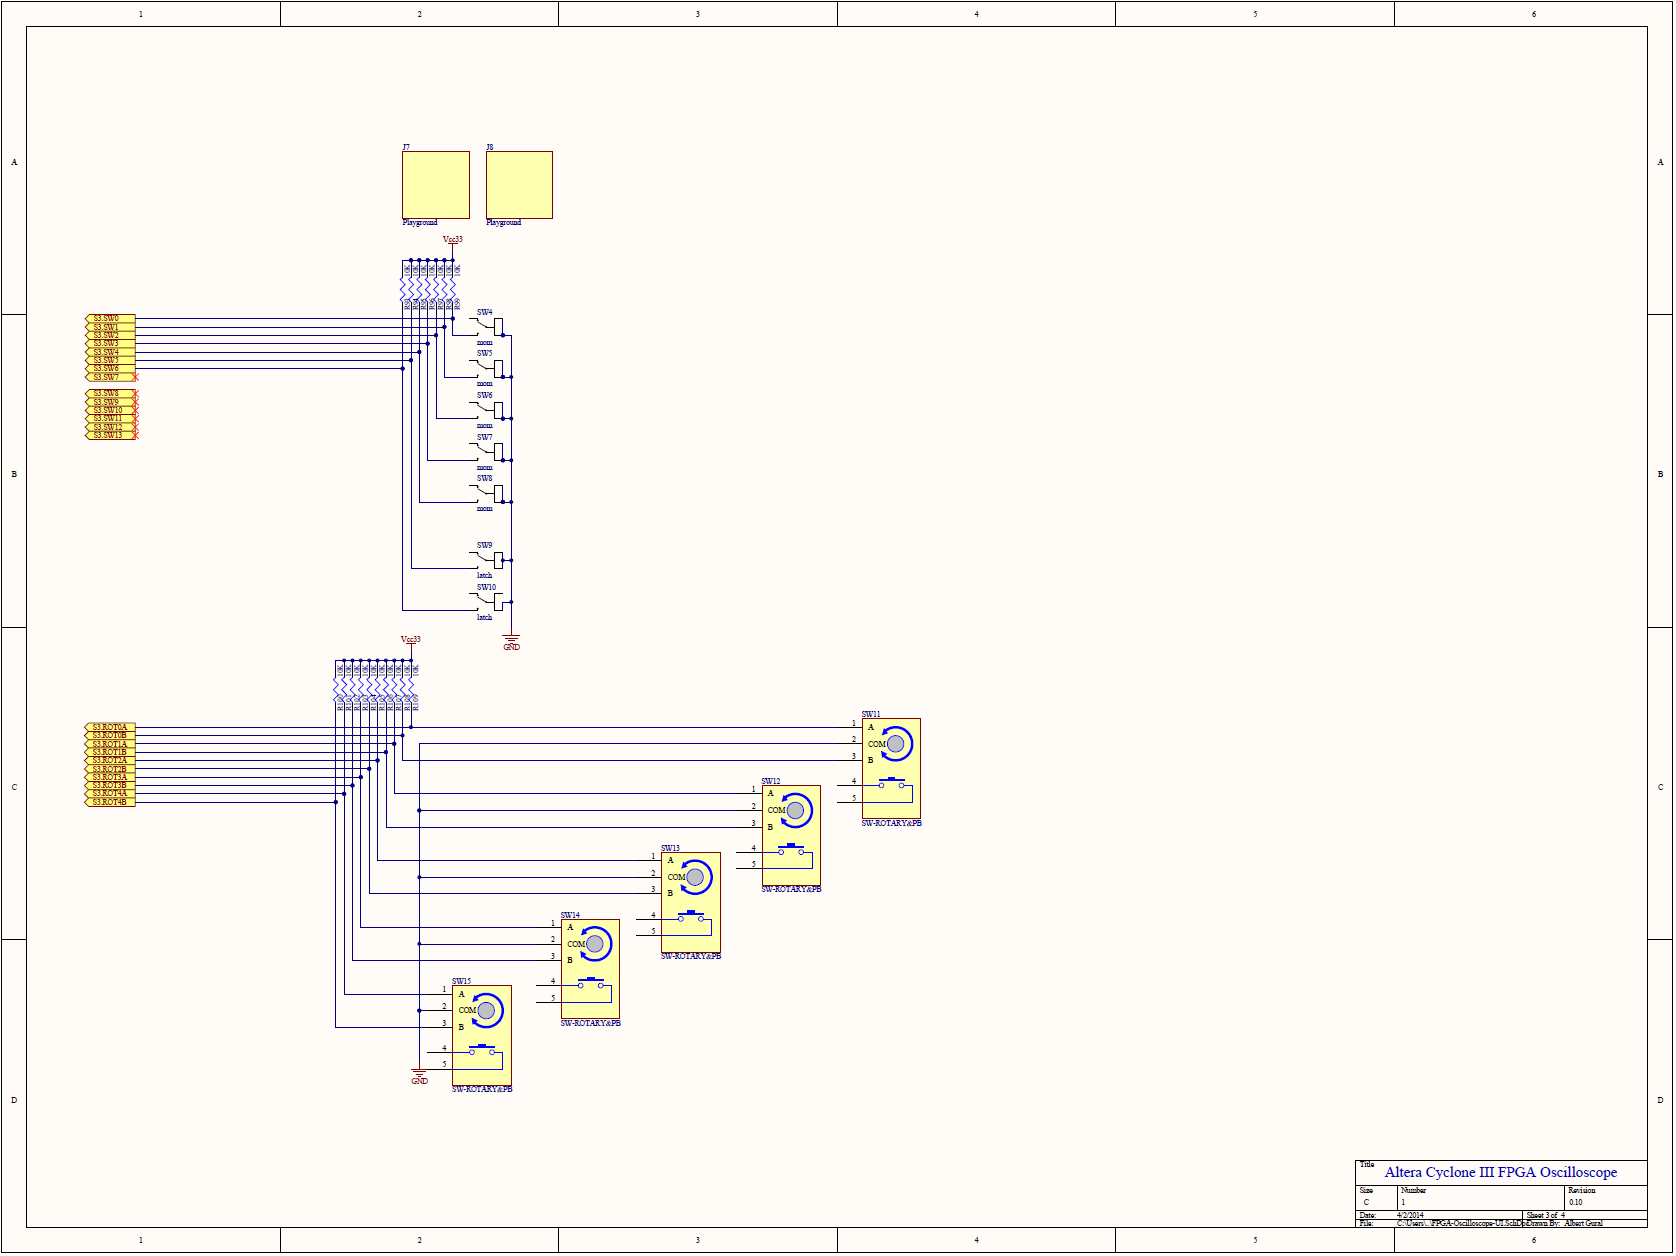
\includegraphics[width=6in]{circuit/switches.png}
		\caption{Switches schematic diagram}
\end{figure}

All of the switches are held high by $1k\Omega$ resistors (resistors in the range of $1k\Omega$ are required due to the low input impedance of the buffers). When the switch closes (or during certain phases of the rotary encoder), the switch terminal is brought from $V_{CC}$ to $GND$. From there, the signals are debounced or decoded in FPGA logic to the soft core CPU.

\begin{figure}[ht!]
    \centering
    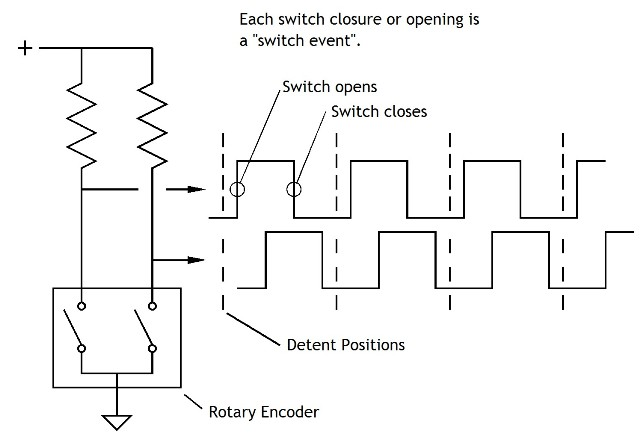
\includegraphics[width=3in]{Timing/encoder.jpg}
		\caption{Rotary encoder timing}
\end{figure}

Rotary encoder timing is shown above. It uses a gray code between two outputs (A/B). Thus, the rotation direction can be detected from the pattern seen.

\section{Board Layout}

Refer to the following diagrams to understand the relationship between the raw board layout, the overarching large-scale hardware modules, and the physical part layout. The first diagram is just the raw board layout. Areas in red are top layer copper and areas in blue are bottom layer copper. The next diagram highlights the major hardware modules and buses. Finally, the third diagram overlays components on top, so the overall design can be intuited.

\begin{figure}[ht!]
    \centering
    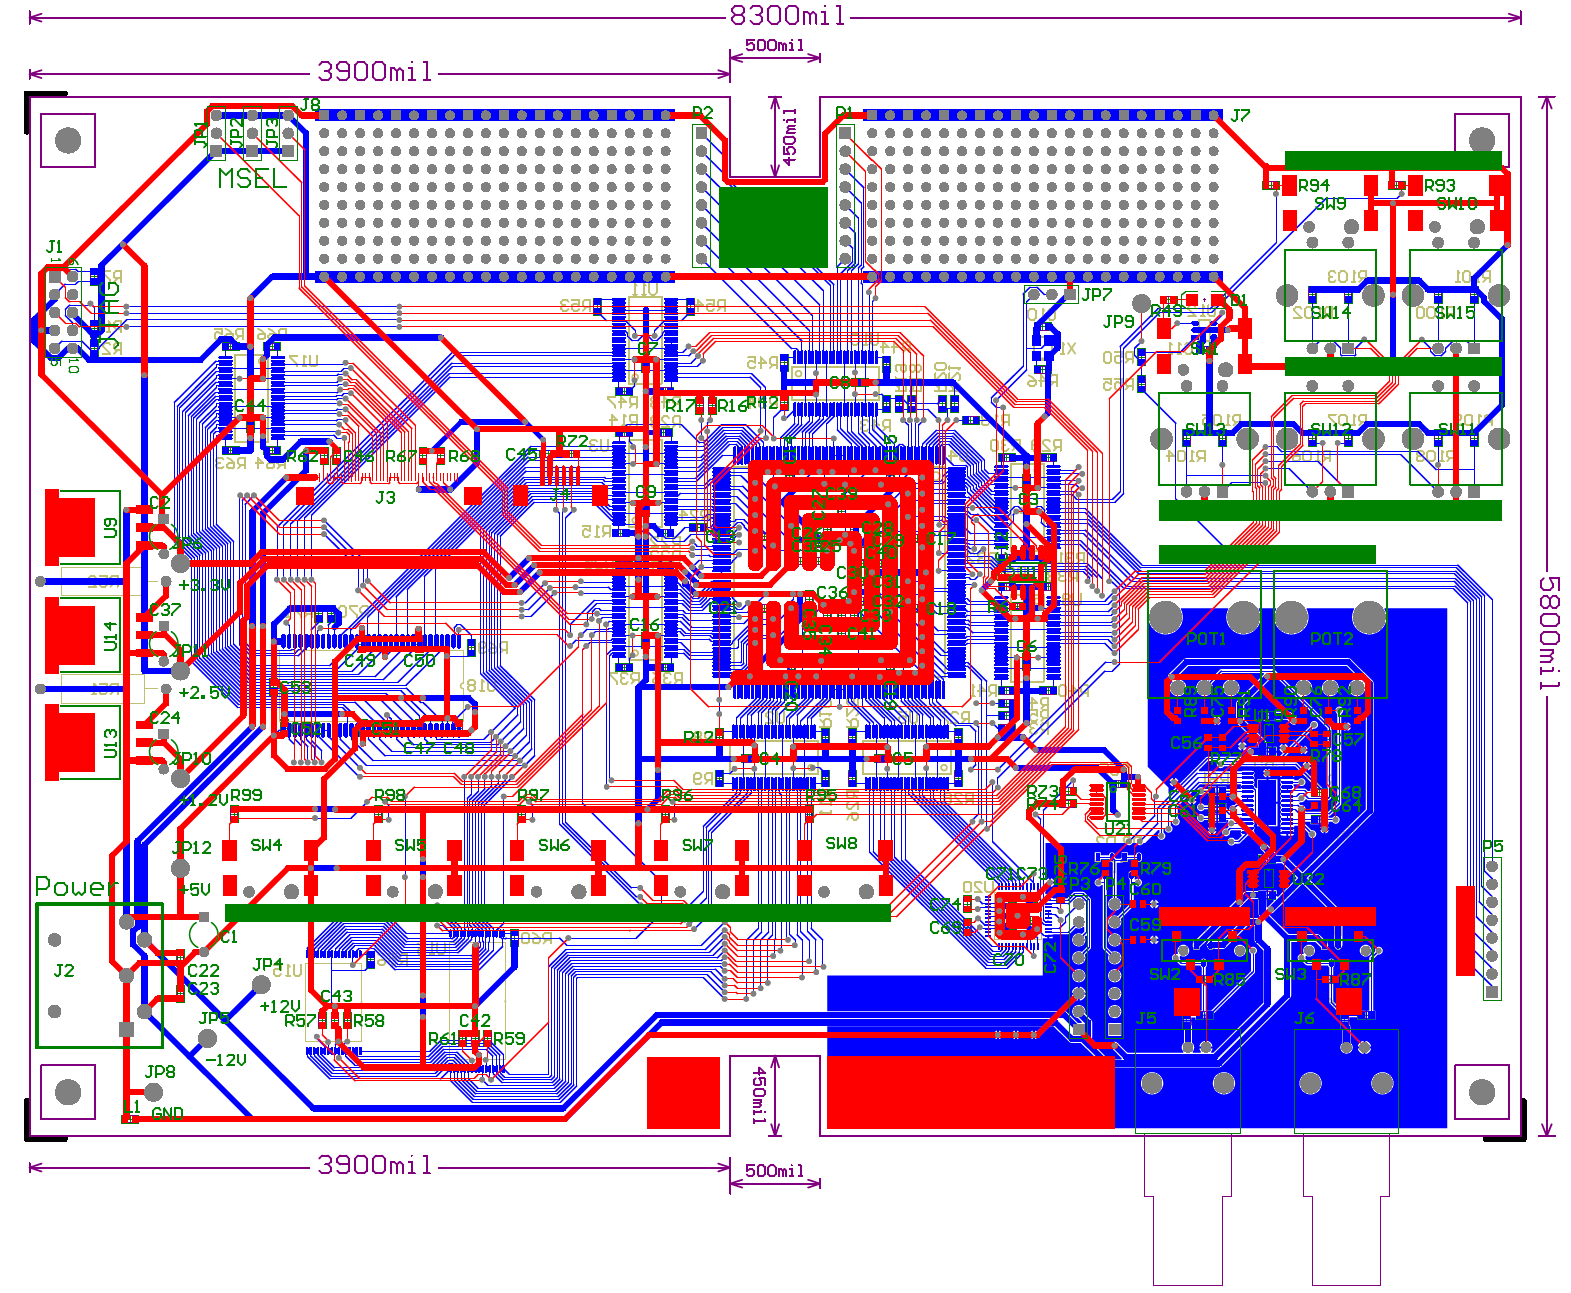
\includegraphics[width=6in]{circuit/board.png}
		\caption{Board layout (raw)}
\end{figure}

\begin{figure}[ht!]
    \centering
    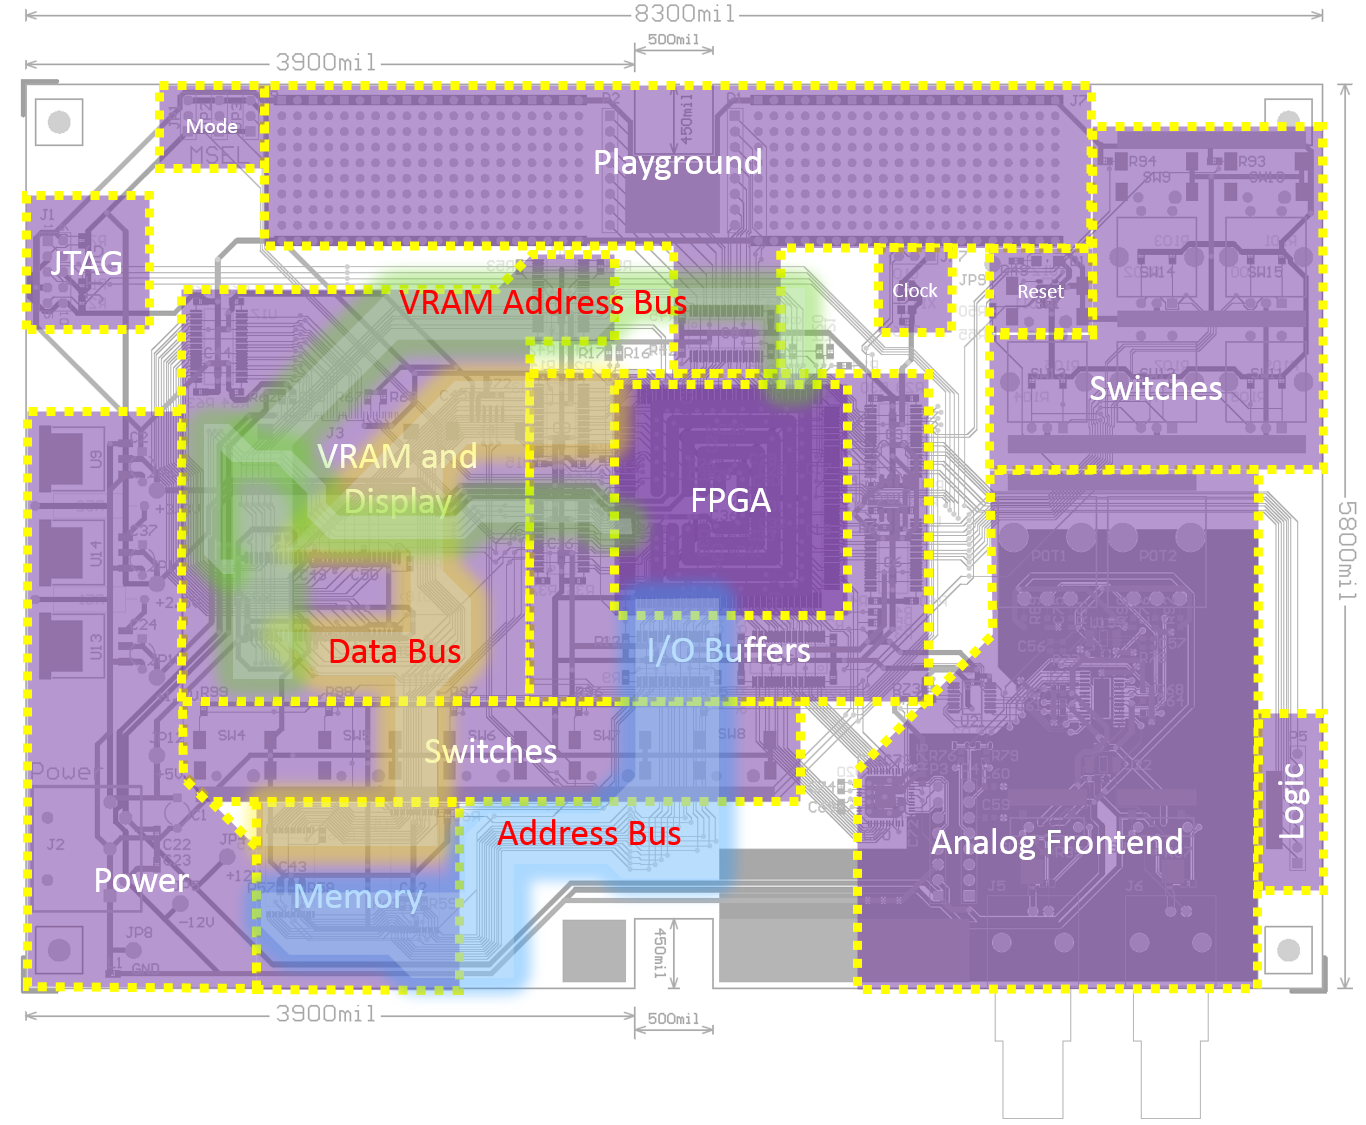
\includegraphics[width=6in]{circuit/board_annotated.png}
		\caption{Board layout with annotations}
\end{figure}

\begin{figure}[ht!]
    \centering
    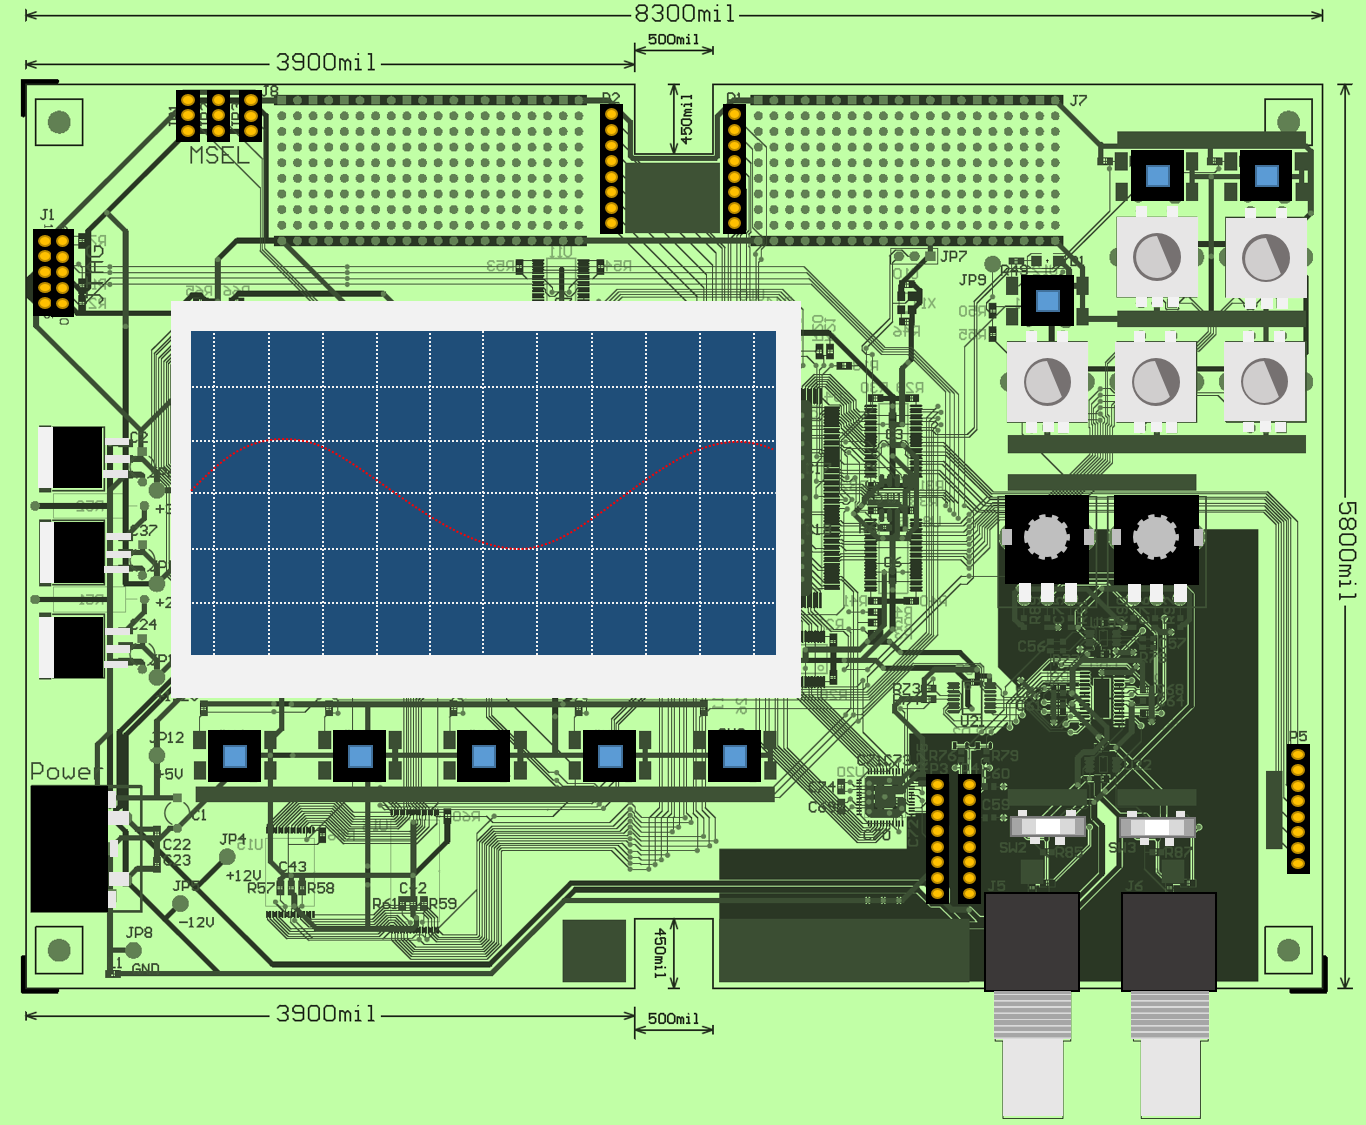
\includegraphics[width=6in]{circuit/board_part_overlay.png}
		\caption{Board layout with top part overlay}
\end{figure}